\documentclass[oneside,14pt]{extarticle}
\usepackage{cmap}
\usepackage[utf8]{inputenc}
\usepackage[english,ukrainian]{babel}
\usepackage{graphicx}
\usepackage{geometry}
\usepackage{listings}
\usepackage{float}
\usepackage{amsmath}
\usepackage{subfig}
\usepackage{tempora}
\geometry{
	a4paper,
	left=20mm,
	right=20mm,
	top=15mm,
	bottom=15mm,
}
\lstset{
	language=c,
	tabsize=4,
	keepspaces,
	showstringspaces=false,
	frame=single,
	breaklines,
	language=C,
}
\graphicspath{ {./pictures} }
\setlength{\parindent}{4em}

\newcommand\subject{Системне адміністрування}
\newcommand\lecturer{професор кафедри ПЗ\\Фечан А.В.}
\newcommand\teacher{професор кафедри ПЗ\\Фечан А.В.}
\newcommand\mygroup{ПЗ-42}
\newcommand\lab{3}
\newcommand\theme{Дозволи та квоти NTFS. Шифрування файлів: EFS}
\newcommand\purpose{Навчитись ефективно налагоджувати систему логічного
	розділення доступу до об’єктів файлової системи в ОС Windows 10; управляти
	квотами на томах NTFS та використовувати шифровану файлову систему EFS}

\begin{document}
\begin{normalsize}
	\begin{titlepage}
		\thispagestyle{empty}
		\begin{center}
			\textbf{МІНІСТЕРСТВО ОСВІТИ І НАУКИ УКРАЇНИ\\
				НАЦІОНАЛЬНИЙ УНІВЕРСИТЕТ "ЛЬВІВСЬКА ПОЛІТЕХНІКА"}
		\end{center}
		\begin{flushright}
			\textbf{ІКНІ}\\
			Кафедра \textbf{ПЗ}
		\end{flushright}
		\vspace{80pt}
		\begin{center}
			\textbf{ЗВІТ}\\
			\vspace{10pt}
			до лабораторної роботи № \lab\\
			\textbf{на тему}: <<\textit{\theme}>>\\
			\textbf{з дисципліни}: <<\subject>>
		\end{center}
		\vspace{80pt}
		\begin{flushright}
			
			\textbf{Лектор}:\\
			\lecturer\\
			\vspace{28pt}
			\textbf{Виконав}:\\
			
			студент групи \mygroup\\
			Коваленко Д.М.\\
			\vspace{28pt}
			\textbf{Прийняв}:\\
			
			\teacher\\
			
			\vspace{28pt}
			«\rule{1cm}{0.15mm}» \rule{1.5cm}{0.15mm} 2024 р.\\
			$\sum$ = \rule{1cm}{0.15mm}……………\\
			
		\end{flushright}
		\vspace{\fill}
		\begin{center}
			\textbf{Львів — 2024}
		\end{center}
	\end{titlepage}
		
	\begin{description}
		\item[Тема.] \theme.
		\item[Мета.] \purpose.
	\end{description}

    \section*{Лабораторне завдання}
	\begin{enumerate}
		\item Створити на томі NTFS нову папку. Дозволити усім користувачам створювати файли і папки у цій папці, але заборонити її видаляти.
		\item Увійти до системи під іншим користувачем та переконатися у неможливості видаляти цю папку, однак маючи
		змогу створювати в ній файли та підпапки. Створити таку підпапку;
		переконатись, що як власник об’єкту цей користувач має право на зміну усіх
		дозволів. Заборонити групі «Administrators» повний доступ до створеної
		підпапки.
		\item Увійти до системи як користувач з адміністративними повноваженнями.
		Переконатись у відсутності доступу до підпапки. Зайти на вкладку "Безпека" властивостей об’єкту. В додаткових
		параметрах безпеки змінити власника папки.
		\item Для приведення налаштування безпеки усіх вкладених субконтейнерів і
		об’єктів до шаблонного зразка батьківської папки використати відмітку
		"Замінити всі дозволи дочірнього…" вкладки "Додатково" додаткових
		параметрів безпеки для папки.
		\item Користувачем з адміністративними правами перейти на вкладку "Квота"
		властивостей NTFS тому. Включити управління квотами у "м’якому" режимі. У
		вікні "Записи квоти" скориставшись меню "Квота" створити
		індивідуальний запис квоти для певного користувача. Увійти до системи під іншим користувачем. Записати на том з квотами
		файли сумарним обсягом більшим від порогу попереджень, але меншим за
		розмір квоти.
		Увійти до системи під третім користувачем. Записати на том з квотами
		файли сумарним обсягом більшим за розмір квоти.
		Користувачем з адміністративними правами переглянути записи квот для
		цього тому. Включити квоти у "жорсткому" режимі.
		Увійти до системи під іншим користувачем. Спробувати записати на том з
		квотами файли сумарним обсягом більшим за розмір квоти. Переконатись у
		неможливості такої операції.
		\item Створити агента відновлення шифрованих даних.
		\item Увійшовши до системи під декількома користувачами зашифруйте по
		одному файлу для кожного користувача. 
	\end{enumerate}

	\section*{Хід роботи}
	
	\begin{figure}[H]
		\centering
		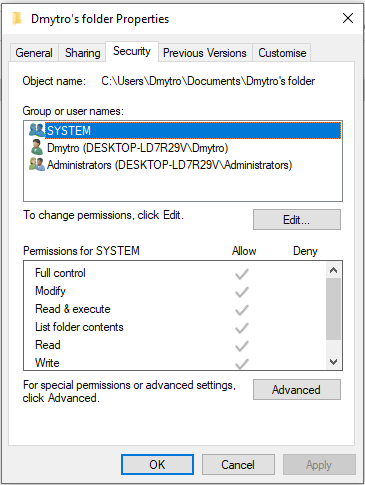
\includegraphics[width=\columnwidth]{1}
		\caption{Вкладка "Безпека" властивостей об'єкту файлової системи}
	\end{figure}
	
	\begin{figure}[H]
		\centering
		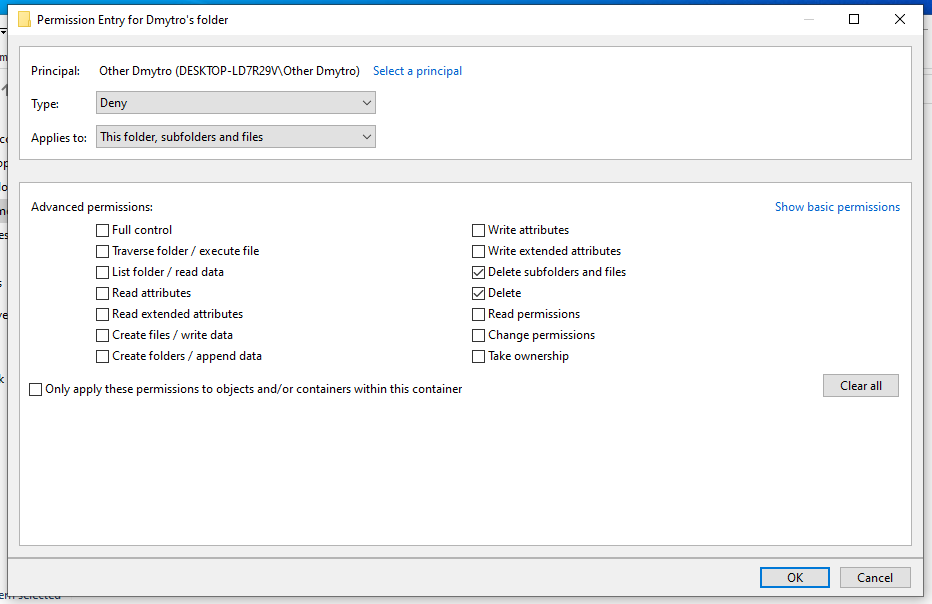
\includegraphics[width=\columnwidth]{2}
		\caption{Встановлення заборони на видалення файлів у папці для всіх користувачів}
	\end{figure}
	
	\begin{figure}[H]
		\centering
		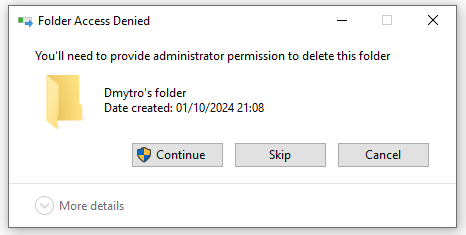
\includegraphics[width=\columnwidth]{3}
		\caption{Заборона на видалення папки в дії}
	\end{figure}
	
	\begin{figure}[H]
		\centering
		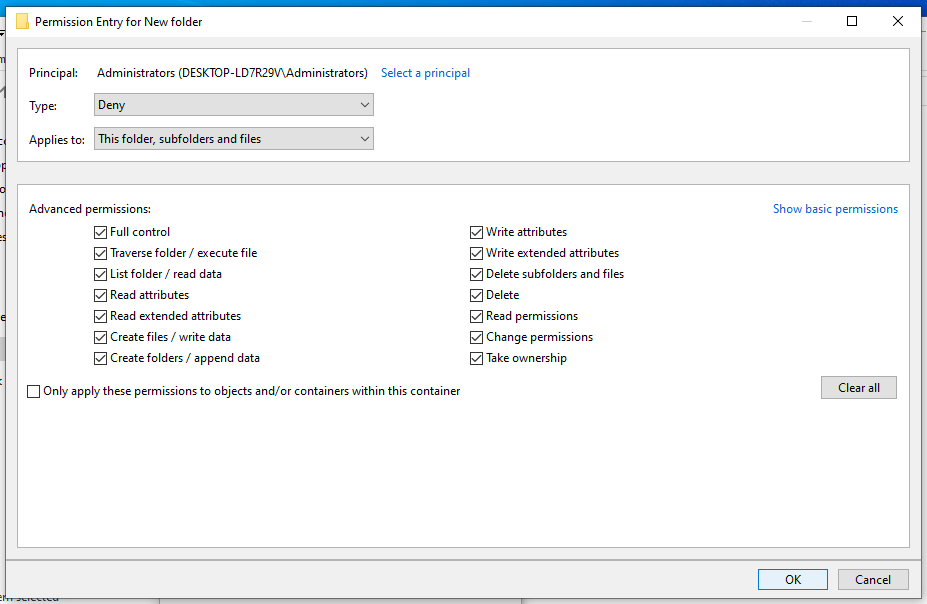
\includegraphics[width=\columnwidth]{4}
		\caption{Повна заборона доступу до папки для адміністраторів}
	\end{figure}
	
	\begin{figure}[H]
		\centering
		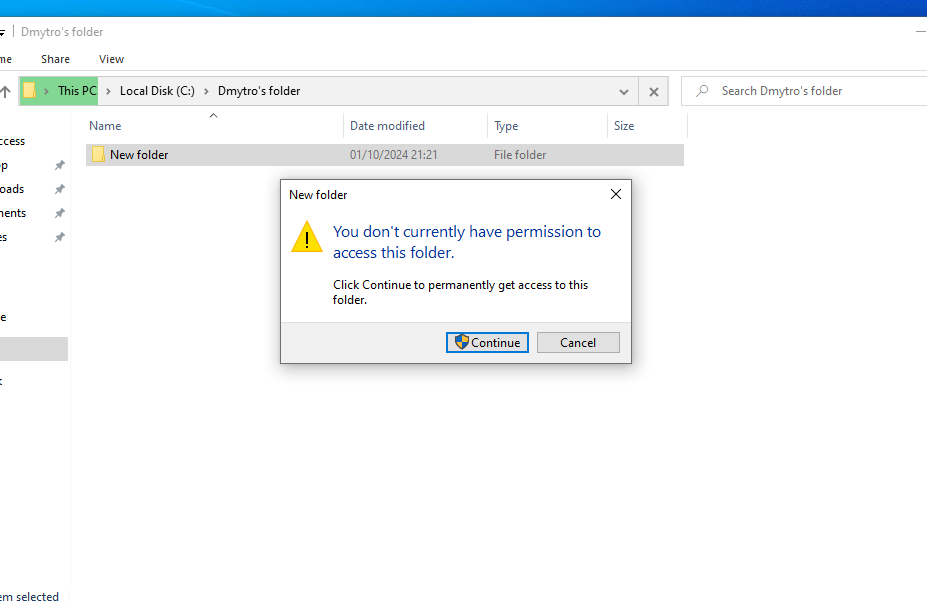
\includegraphics[width=\columnwidth]{5}
		\caption{Повна заборона в дії}
	\end{figure}
	
	\begin{figure}[H]
		\centering
		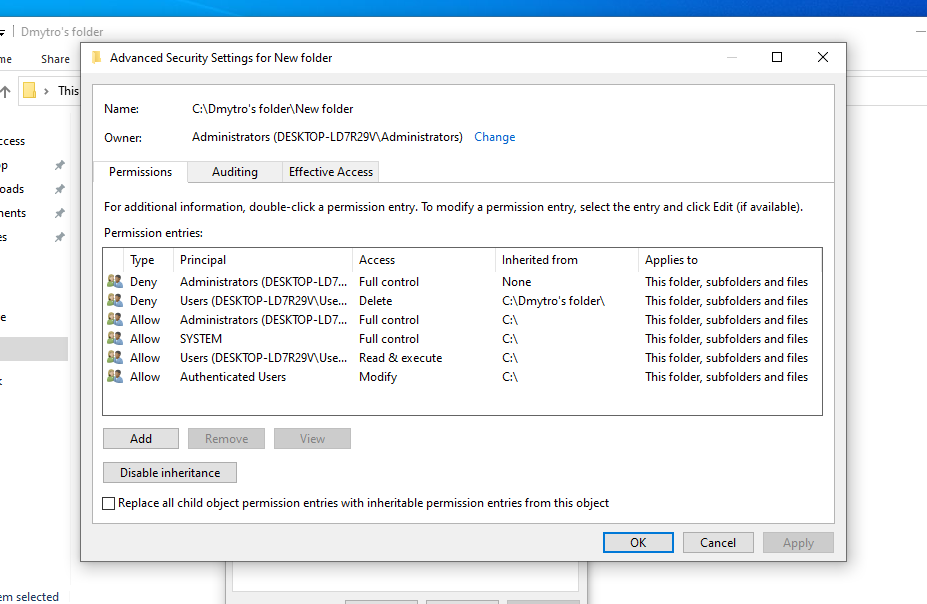
\includegraphics[width=\columnwidth]{6}
		\caption{Зміна власника папки}
	\end{figure}
	
	\begin{figure}[H]
		\centering
		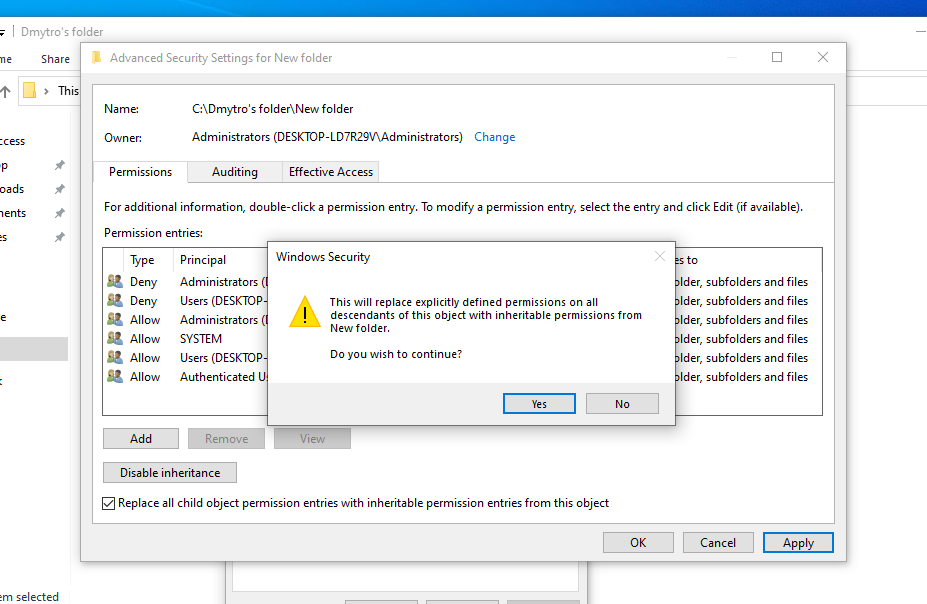
\includegraphics[width=\columnwidth]{7}
		\caption{Приведення налаштування безпеки усіх вкладених субконтейнерів і
			об’єктів до шаблонного зразка батьківської папки}
	\end{figure}
	
	\begin{figure}[H]
		\centering
		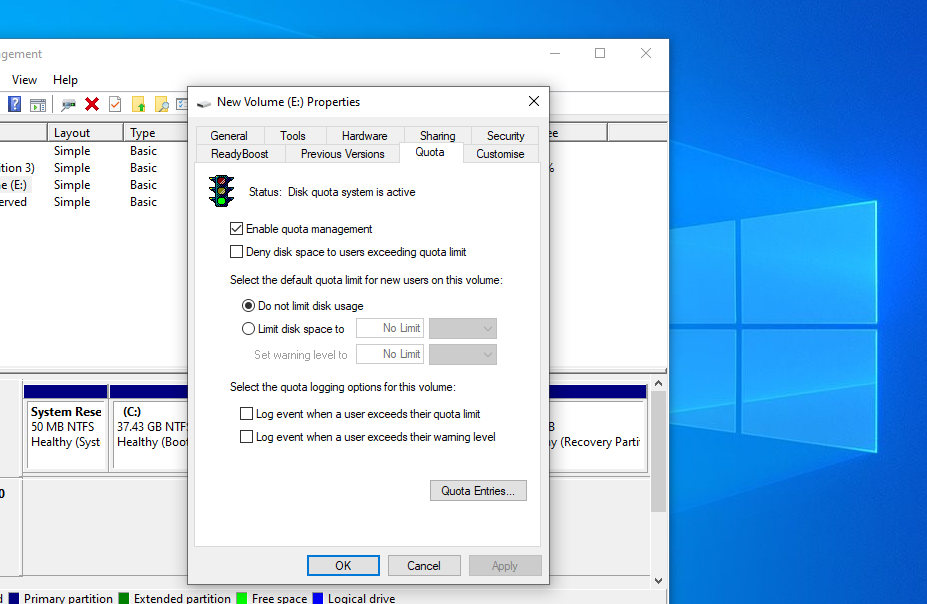
\includegraphics[width=\columnwidth]{8}
		\caption{Увімкнення керування квотами}
	\end{figure}
	
	\begin{figure}[H]
		\centering
		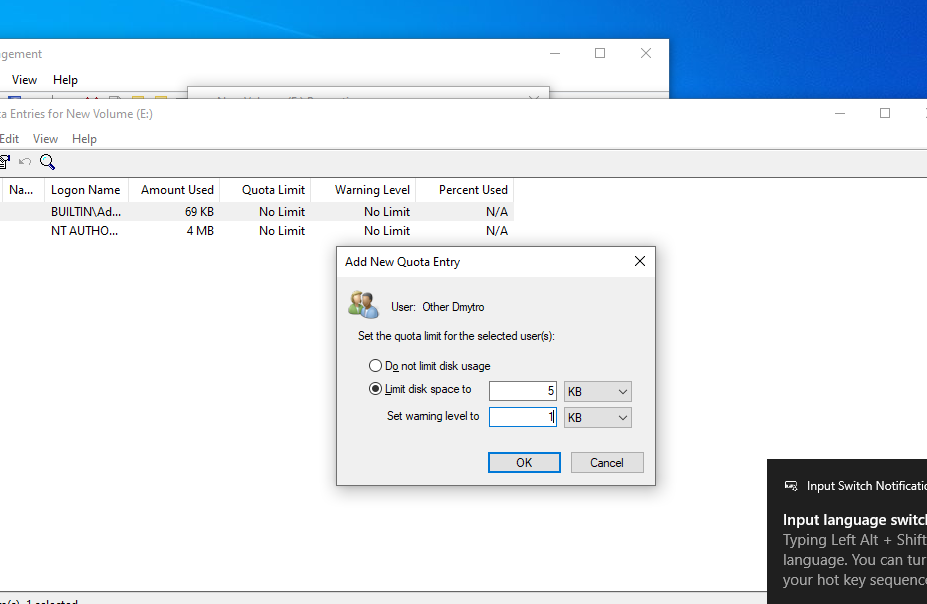
\includegraphics[width=\columnwidth]{9}
		\caption{Створення квоти для користувача}
	\end{figure}
	
	\begin{figure}[H]
		\centering
		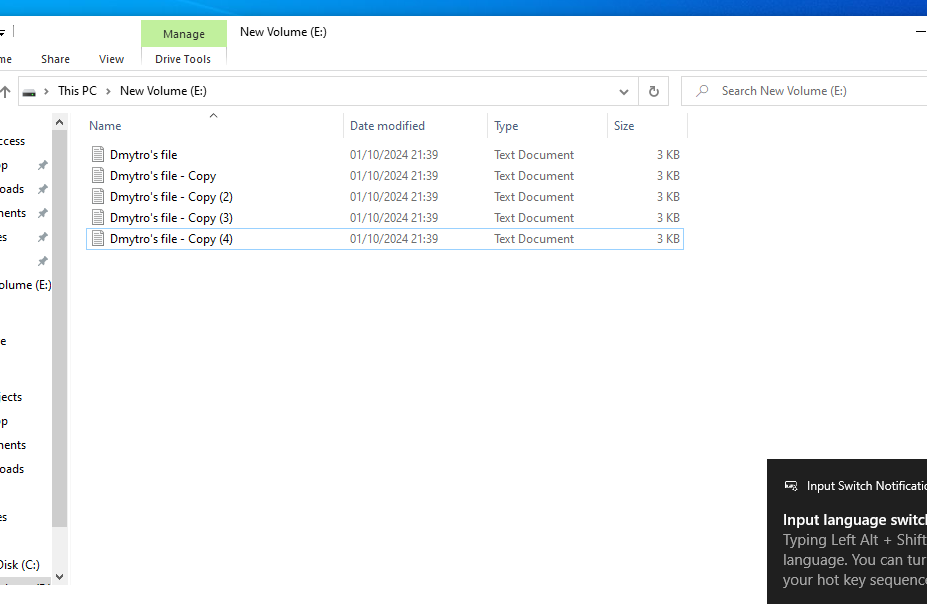
\includegraphics[width=\columnwidth]{10}
		\caption{Запис файлів}
	\end{figure}
	
	\begin{figure}[H]
		\centering
		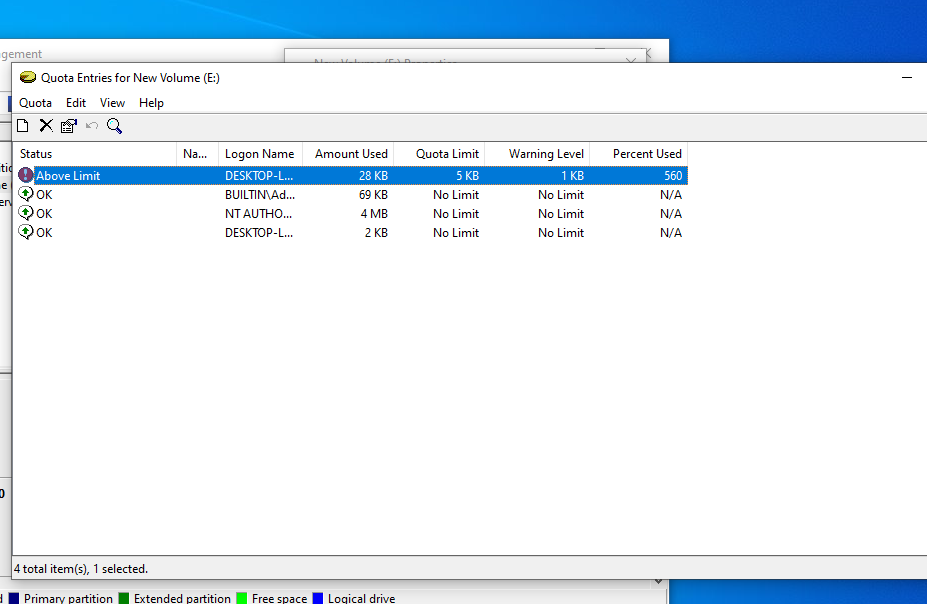
\includegraphics[width=\columnwidth]{11}
		\caption{Повідомлення про перевищення ліміту}
	\end{figure}
	
	\begin{figure}[H]
		\centering
		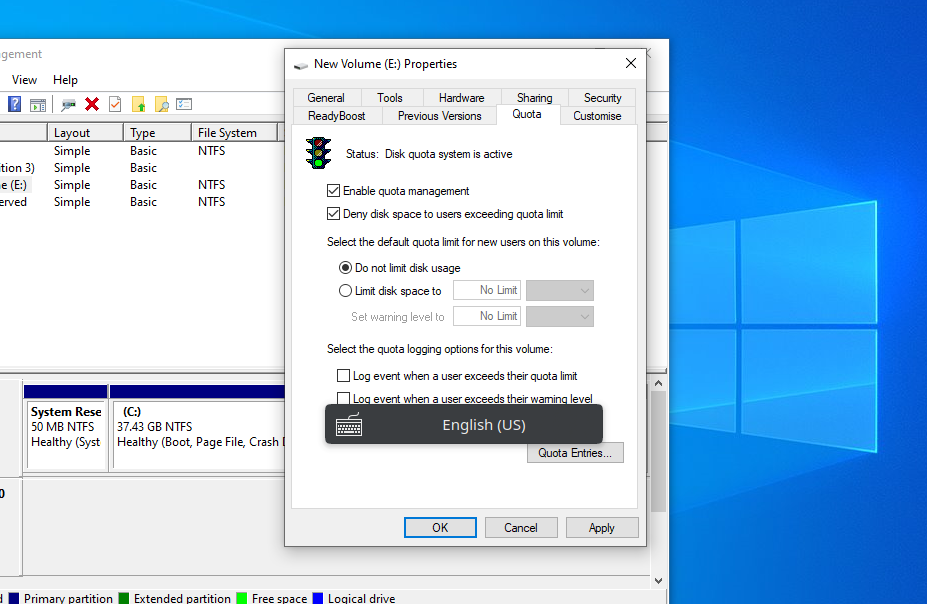
\includegraphics[width=\columnwidth]{12}
		\caption{Встановлення жорсткого обмеження}
	\end{figure}
	
	\begin{figure}[H]
		\centering
		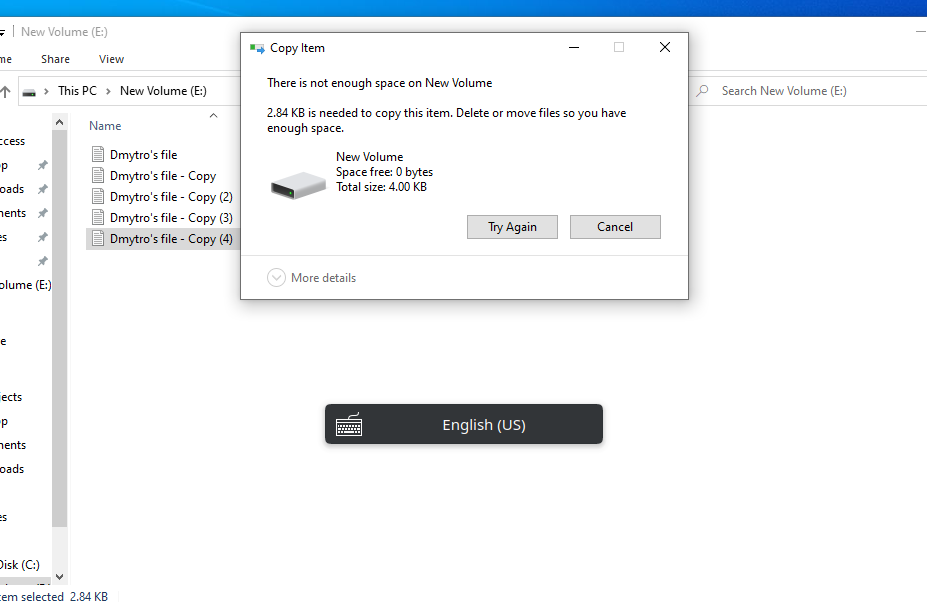
\includegraphics[width=\columnwidth]{13}
		\caption{Результат встановлення обмеження}
	\end{figure}
	
	\begin{figure}[H]
		\centering
		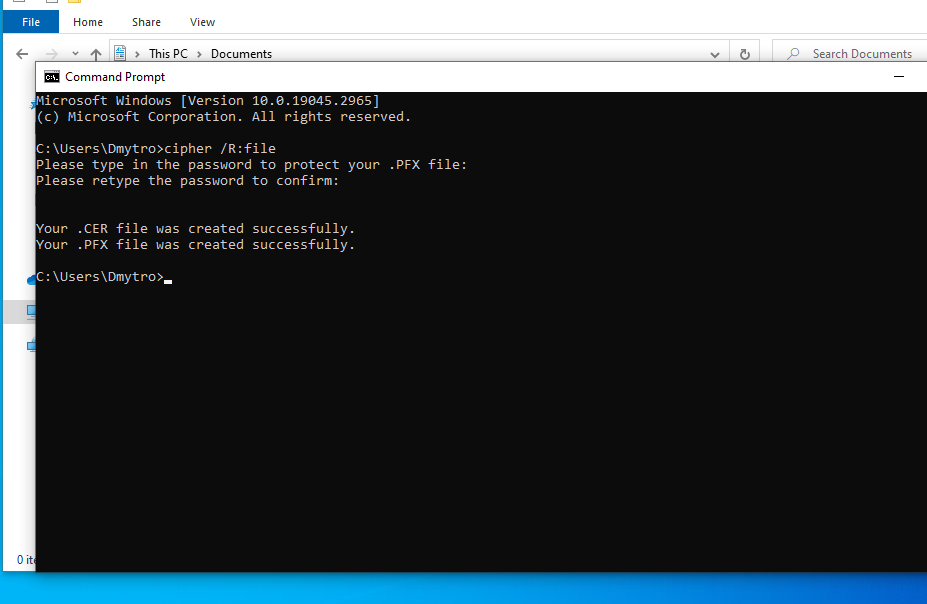
\includegraphics[width=\columnwidth]{14}
		\caption{Створення ключів}
	\end{figure}
	
	\begin{figure}[H]
		\centering
		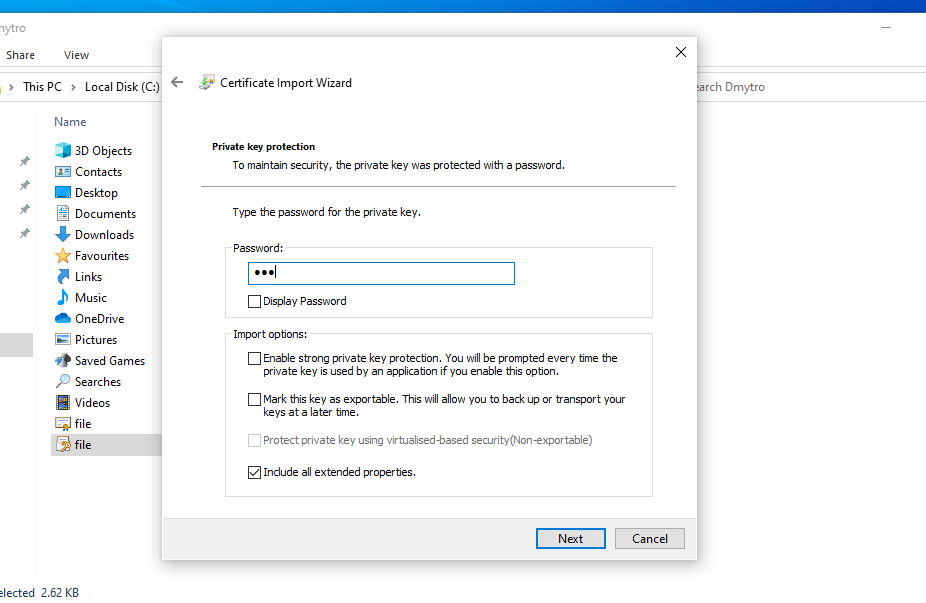
\includegraphics[width=\columnwidth]{15}
		\caption{Імпорт сертифікатів}
	\end{figure}
	
	\begin{figure}[H]
		\centering
		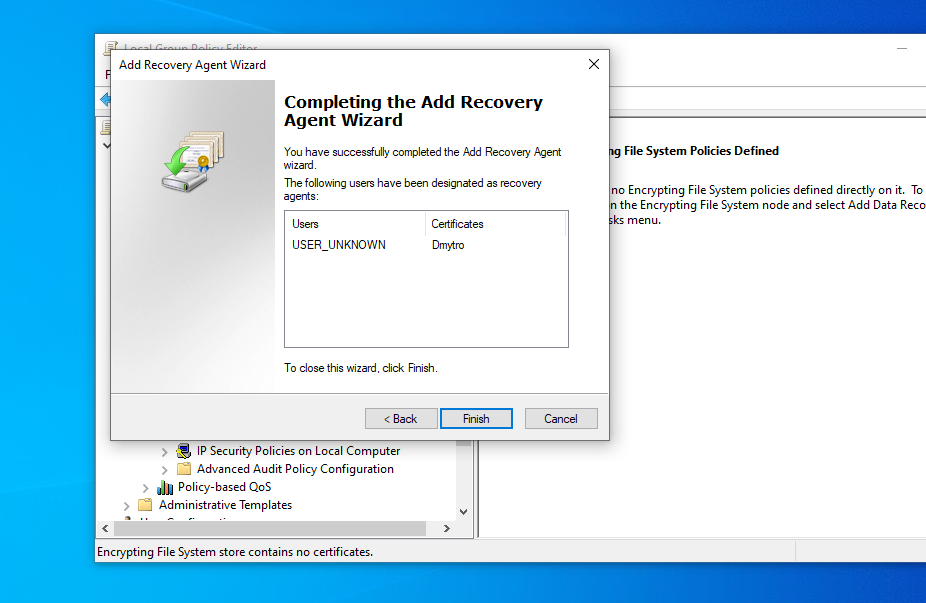
\includegraphics[width=\columnwidth]{16}
		\caption{Створення агента відновлення}
	\end{figure}
	
	\begin{figure}[H]
		\centering
		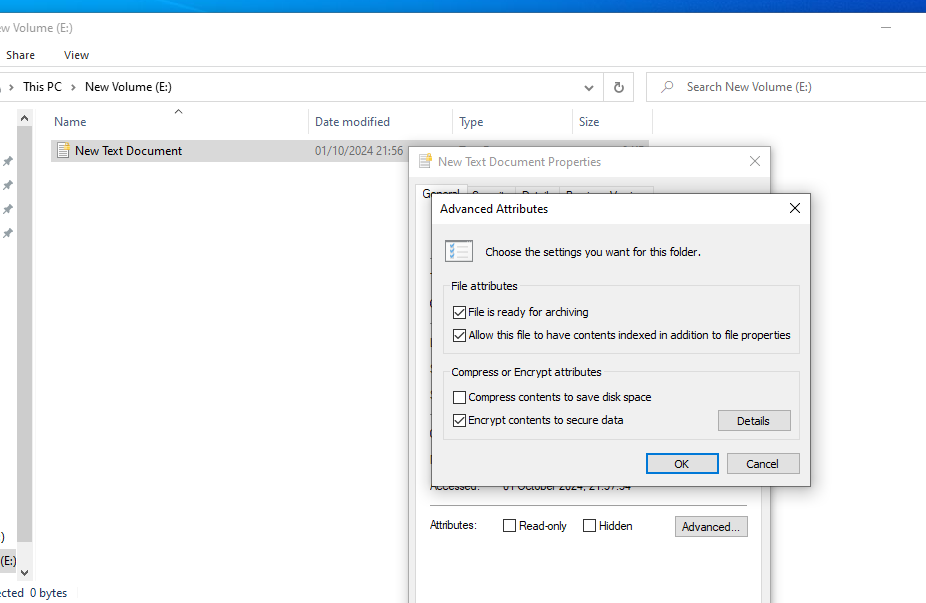
\includegraphics[width=\columnwidth]{17}
		\caption{Шифрування файлу}
	\end{figure}
	
	\begin{figure}[H]
		\centering
		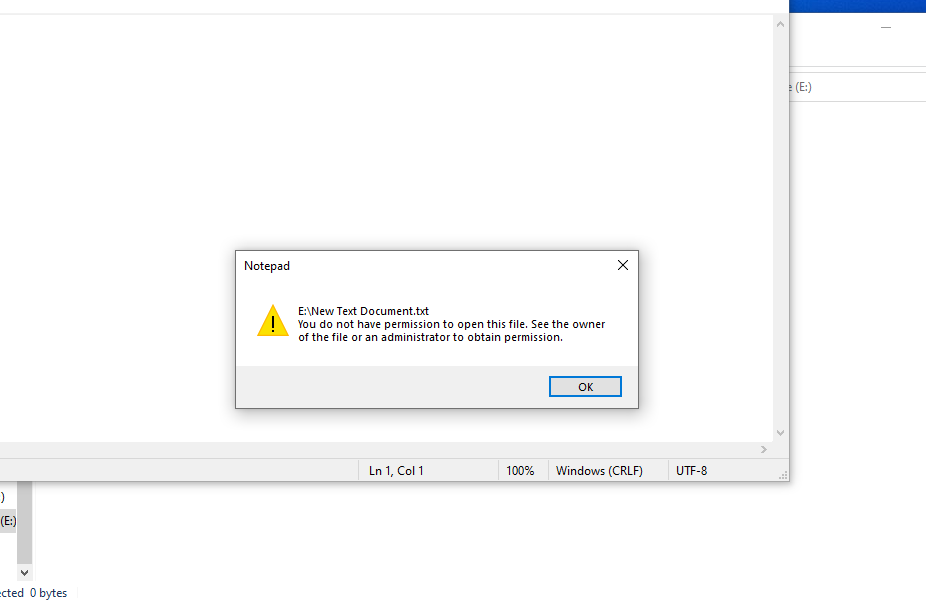
\includegraphics[width=\columnwidth]{18}
		\caption{Результат шифрування файлу}
	\end{figure}
	
	\section*{Висновки}
	Під час виконання лабораторної роботи я навчився ефективно налагоджувати систему логічного
	розділення доступу до об’єктів файлової системи в ОС Windows 10; управляти
	квотами на томах NTFS та використовувати шифровану файлову систему EFS.
		    
\end{normalsize}
\end{document}
